\documentclass{article}
\usepackage{spconf,amsmath,graphicx}
\usepackage{subcaption}
\usepackage{breqn}
\usepackage{amsmath}
\usepackage{pdflscape}

\usepackage{amssymb}
\usepackage{graphicx}
\usepackage{caption}
\usepackage{subcaption}

\usepackage{url}
\usepackage{amsmath}
\usepackage{graphicx,psfrag,epsfig,color,comment,array}

\usepackage{epsf}
\usepackage{graphicx,psfrag,color,pstcol,pst-grad}
\usepackage{pst-blur}
\usepackage{amsmath,amssymb}
\usepackage{latexsym}
\usepackage{calc}

\usepackage{multicol,xspace,comment,epsfig,array,comment}



% Example definitions.
% --------------------
\def\x{{\mathbf x}}
\def\L{{\cal L}}

% Title.
% ------
\title{Epileptiform Spike Detection via Convolutional Neural Networks}

\name{\small Alexander Rosenberg Johansen$^{a,b}$, Jing Jin$^b$, Tomasz Maszczyk$^b$, Justin Dauwels$^b$, Sydney S.~Cash$^c$, M.~Brandon Westover$^c$}

\address{\small $^a$ Technical University of Denmark, DTU Compute, Lyngby, Denmark\\
         \small $^b$ Nanyang Technological University, School of Electrical and Electronic Engineering, Singapore\\
         \small $^c$ Massachusetts General Hospital Neurology Department, and Harvard Medical School, USA\\}

% --------------

\begin{document}
%\ninept
%
\maketitle
%
\begin{abstract}
The EEG of epileptic patients often contains sharp waveforms called ``spikes", occurring between seizures.
Detecting such spikes is crucial for diagnosing epilepsy.
In this paper, we develop a convolutional neural network~(CNN) for detecting spikes in EEG of epileptic patients in an automated fashion.~The CNN has a convolutional architecture with filters of various sizes applied to the input layer, leaky ReLUs as activation functions, and a sigmoid output layer.
Balanced mini-batches were applied to handle the imbalance in the data set.
Leave-one-patient-out crossvalidation was carried out to test the CNN and benchmark models on EEG data of five epilepsy patients.~We achieved 0.947 AUC for the CNN, while the best performing benchmark model, Support Vector Machines with Gaussian kernel, achieved
an AUC of 0.912.

\end{abstract}
%
\begin{keywords}
Epilepsy, Spike detection, EEG, Deep learning, Convolutional neural network
\end{keywords}
%
\section{Introduction}
\label{sec:intro}
Epilepsy refers to a group of chronic brain disorders characterized by recurrent seizures, affecting approximately 65 million people worldwide~\cite{EFA2014epilepsy}.
Electroencephalography~(EEG) is the primary diagnostic test for epilepsy, which provides a continuous measure of cortical function with excellent temporal resolution.
Significant efforts are spent on interpreting EEG data for clinical purposes.~In current clinical practice, visual inspection and manual annotation are still the gold standard for interpreting EEG, which is tedious and ultimately subjective.~In addition, experienced electroencephalographers are in short supply~\cite{racette2014supply}.
As a result, a great need exists for automated systems for EEG interpretation.\\

The finding of primary importance for the diagnosis for epilepsy is the presence of interictal discharges, also known as ``spikes" and ``sharp waves", hereafter referred to collectively simply as ``spike(s)".~Automated spike detection would enable wider availability of EEG diagnostics and more rapid referral to qualified physicians who can provide further medical
investigation and interventions.~However, spikes are difficult to detect in a consistent manner due to the large variability of spike waveforms between patients among other factors~\cite{jin2014spikegui}.
Great attempts have been made to detect spikes by general classifications such as mimetic, linear predictive, and template based methods~\cite{wilson2002spike}.~Many recent spike detection algorithms combine multiple methodologies, such as local context~\cite{gotman1992state,guedes1983spike,wilson1999spike},
morphology~\cite{gotman1991state,guedes1983spike,wilson1999spike,faure1985attributed,davey1989expert,webber1994practical},
field of spike~\cite{gotman1991state,wilson1999spike,gabor1992automated,webber1994practical,ramabhadran1999automated},
artifact rejection~\cite{gotman1991state,guedes1983spike,wilson1999spike}, and temporal and spatial contexts~\cite{gotman1991state,ramabhadran1999automated,black2000real}.~Unfortunately, none of them are universally accepted or tested on a significantly large dataset of patients and spikes. To date, no algorithmic approach has overcome these challenges to yield expert-level detection of spikes~\cite{jin2014spikegui}.\\

In this study, we analyze the scalp EEG recordings of five patients diagnosed with epilepsy. Suspected interictal epileptiform spikes were cross-annotated by two neurologists.~We applied convolutional neural networks~(CNNs) to learn the discriminative features of spikes.~CNNs are statistical models incorporating prior knowledge about the discriminative features of spikes.~CNNs are commonly applied for finding local pixel dependencies~\cite{NIPS2012_4824}.
Furthermore, CNNs have been proven successful in surpassing human accuracy in image recognition tasks~\cite{DBLP:journals/corr/HeZR015}, time-series tasks for text analysis~\cite{DBLP:journals/corr/ZhangL15} and biological sequences~\cite{sonderby2015convolutional}.~In addition, CNNs possess much fewer connections compared to a fully-connected neural network, due to the sparsity and the parameter sharing across the filters. Nevertheless, the computational complexity remains a key challenge to implementing CNNs.~To address this issue, we utilize Graphical Processing Units~(GPUs) and high performance libraries for modeling CNNs. \\

We benchmarked the CNN approach with several standard classification methods.~Leave-one-patient-out crossvalidation was conducted to generate the receiver operating characteristic~(ROC) curve for each model, with the average area-under-the-curve~(AUC) as the benchmark criterion. We achieved 0.947 AUC for the CNN, while the best performing benchmark model, Support Vector Machines with Gaussian kernel, achieved an AUC of 0.912.
\\

This paper is organized as follows. In Section 2, we provide information on the EEG data considered in this study. We also elaborate on the design of the CNN model. In Section 3, we provide results for the CNN approach and four standard classifiers.~In Section 4, we offer concluding remarks and ideas for future research. \\

\section{Methods}
\subsection{Epileptiform EEG}
We analyzed the scalp EEG recordings of five patients with known epilepsy. Each EEG data lasts 30~minutes recorded from 19 standard 10-20 scalp electrodes.~The sampling rate is 128Hz. A high-pass filter at 1Hz was applied to remove the baseline drifts. A notch filter centered at 60Hz was applied to remove the power line interference.~The common average referencing montage was applied to remove the common EKG artifacts.\\

As shown in Fig. \ref{fig:waveforms}a, interictal epileptiform spikes are morphologically defined events with an outstanding sharp peak distinguishable from the background fluctuations~(see Fig.\ref{fig:waveforms}b). Spikes were cross-annotated independently by two neurologists, and extracted with a fixed duration of 0.5~s. In order to reduce the computational load, we randomly sampled 1,500 spikes and 150,000 background waveforms from each subject.~Leave-one-patient-out crossvalidation was conducted to evaluate the CNN model. Moreover, 10\% of the training data was further extracted under stratified sampling for validation, in order to tune the CNN model.\\

\begin{figure}[!tbh]
        \centering
        \begin{subfigure}[b]{.22\textwidth}
            \centering
            \setlength\fboxsep{0pt}
            \setlength\fboxrule{0.pt}
            \fbox{\includegraphics[trim = 50mm 95mm 45mm 90mm, clip, width=1\textwidth]{spike.pdf}}
            \caption{}
        \end{subfigure}
        \hspace{.1in}
        \begin{subfigure}[b]{.22\textwidth}
            \centering
            \setlength\fboxsep{0pt}
            \setlength\fboxrule{0.pt}
            \fbox{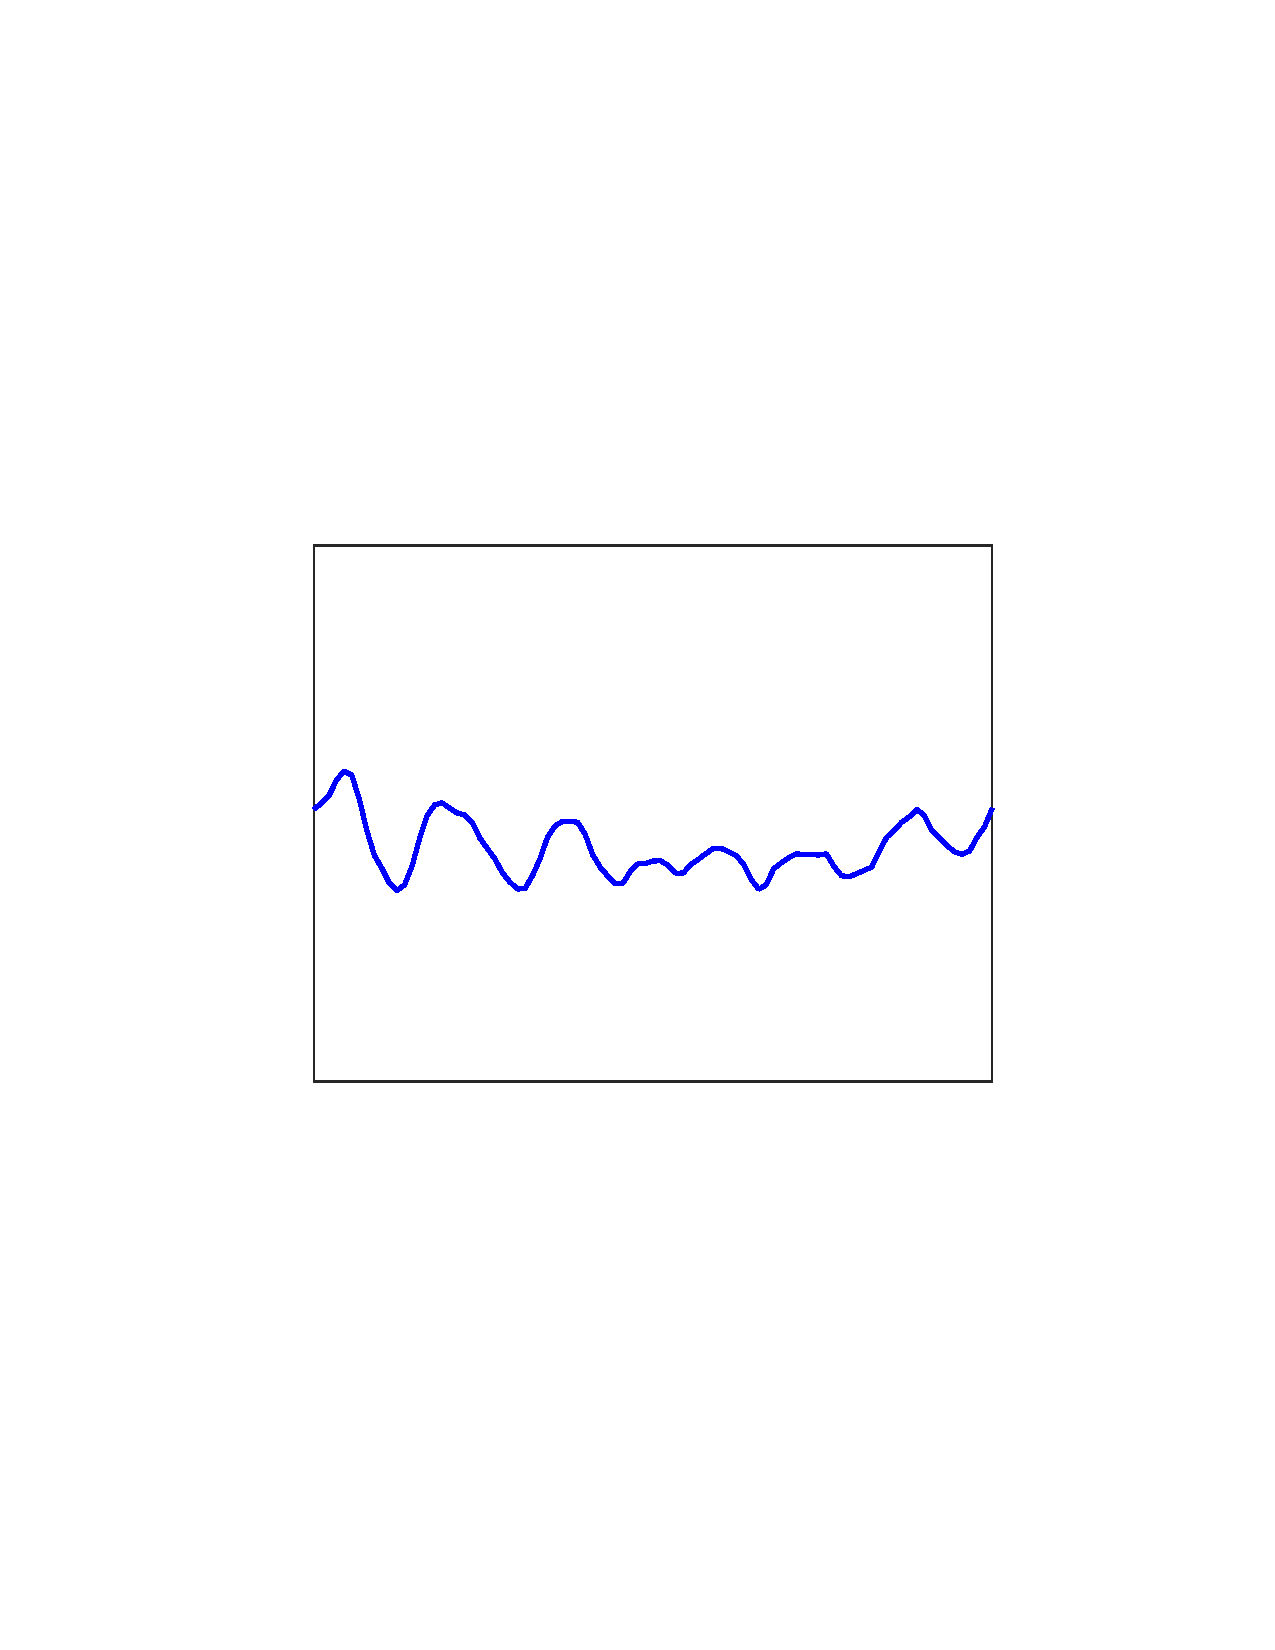
\includegraphics[trim = 50mm 95mm 45mm 90mm, clip, width=1\textwidth]{BG.pdf}}
            \caption{}
        \end{subfigure}

        \caption{Illustration of (a) an interictal epileptiform spike, and (b) a background waveform.}
        \label{fig:waveforms}
\end{figure}


\subsection{Convolutional Neural Networks}

The problem of spike detection is typically ill-posed,~i.e., there are many models which fit the training patients or spikes well but do not generalize well.
In other words, there is often not sufficient training data to allow accurate estimation of class probabilities throughout the input space.~Convolutional neural networks~(CNNs)~\cite{lawrence1997face} are suitable for such scenario, since they incorporate constraints and can achieve some degree of shift and deformation invariance.~The architecture of a CNN~(see Fig.~\ref{fig:CNN}) typically contains multiple layers: convolutional layers, dense layers, and an output layer.
We applied the backpropagation algorithm to train the CNN. In this way, we can extract both low-level and high-level features from the input layer.

\begin{figure}[htb]
    \centering
    \setlength\fboxsep{0pt}
    \setlength\fboxrule{0.pt}
    \fbox{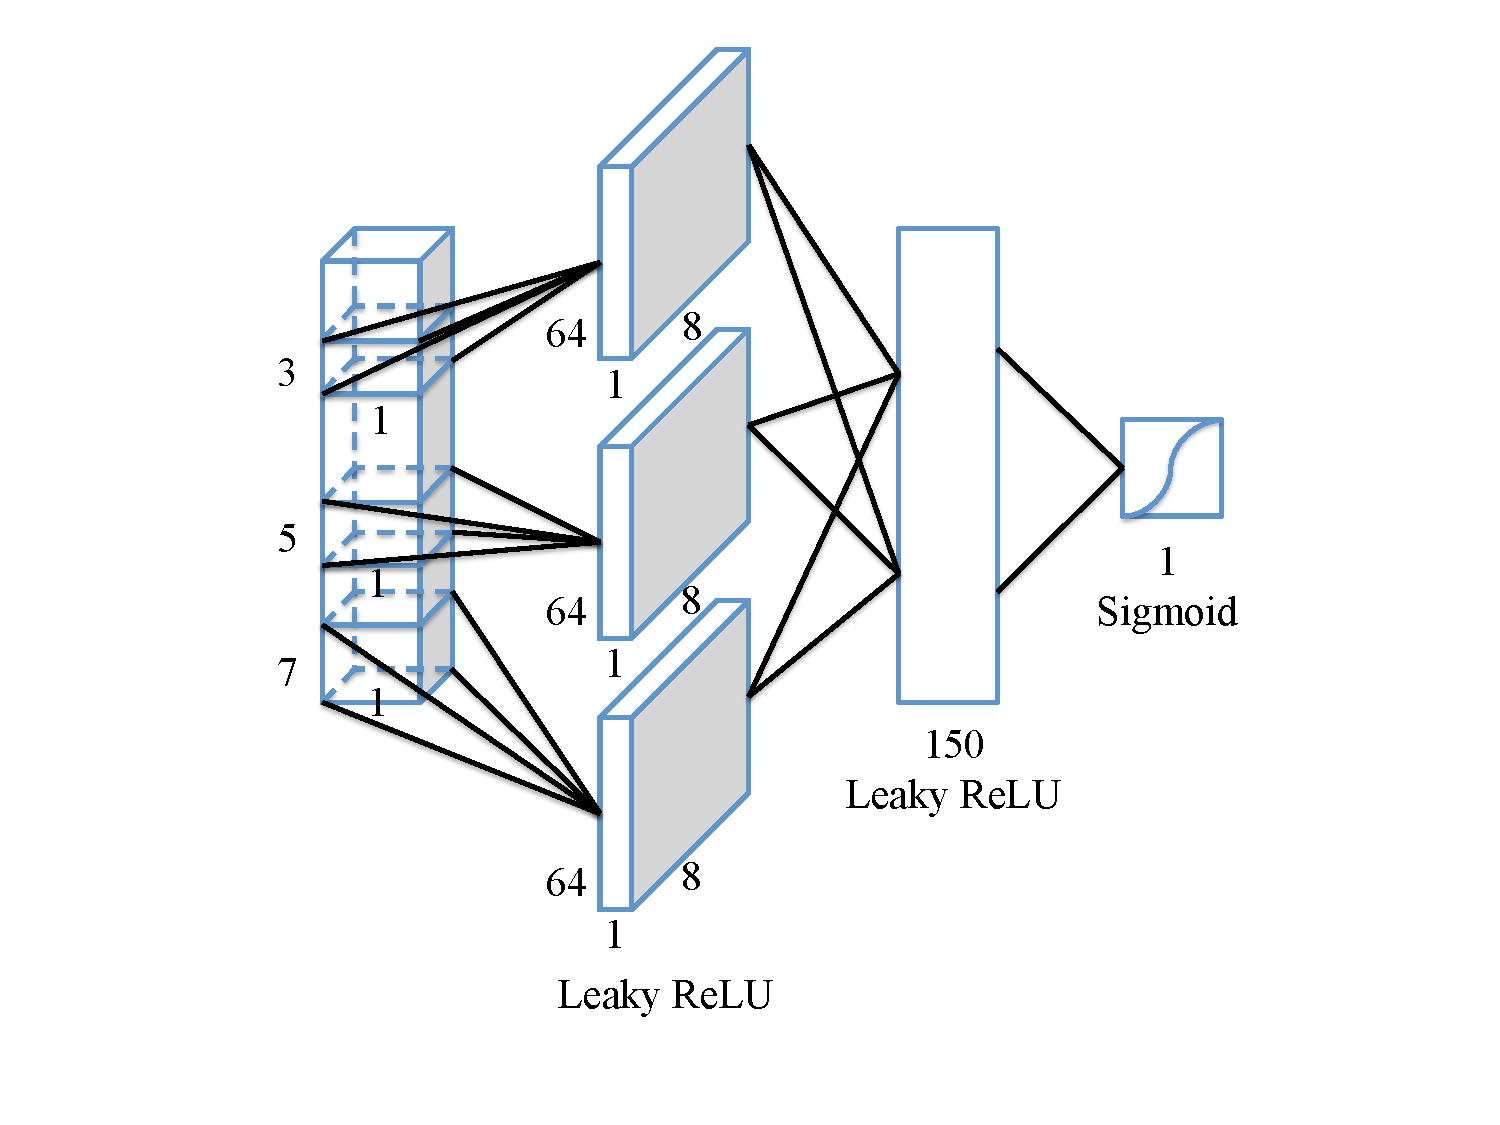
\includegraphics[trim = 45mm 16mm 44mm 8mm, clip, width=.45\textwidth]{CNN.pdf}}
    \caption{The architecture of a the CNN model applied.}
    \label{fig:CNN}
\end{figure}

\subsubsection{Activation function}
\label{ssec:leakyrelus}
In computational networks, the activation function defines the output of a layer given an input or a set of inputs.
Nonlinear activation functions are commonly used in neural networks to improve the learning capacity and system robustness for nontrivial problems.~Let us denote the output of layer $\ell$ as $h_\ell$~(with $h_0$ the input layer), $\Theta_{\ell+1}$ as the weight matrix of layer $\ell$$+$$1$, and $z_{\ell+1}$ as the linear combination of the weighted input to each neuron.~The output of layer $\ell$$+$$1$ is computed as follows:
$$
z_{\ell+1} = h_\ell \Theta_{\ell+1},
$$
$$
h_{\ell+1} = a(z_{\ell+1}),                    \eqno{(1)}
$$
The activation function is denoted by $a(z)$. The most commonly used nonlinear activation functions in neural networks are the Logistic Sigmoid $a(z)=1/(1+e^{-z})$ and the Hyperbolic Tangent $a(z)=(e^z-e^{-z})/(e^z+e^{-z})$.
Non-saturating activation functions such as the Rectifier Linear Unit~(ReLU) with $a(z) = \max(0,~z)$ have become more popular for their non-vanishing gradients and computational efficiency~\cite{NIPS2012_4824}.~However, the ReLU also suffers from ``dead'' gradients,~i.e.~from large gradients that may deactivate the neurons, and further disable the network.~In order to avoid such problems, we applied the Leaky ReLU~\cite{DBLP:journals/corr/HeZR015} as our activation function in CNN, which is defined as:
$$
a(z) = \max(\alpha z, \ z),  \eqno{(2)}
$$
with $\alpha=0.1$.~``Leaky" refers to the additional slope when $a(z)<0$.

\subsubsection{The convolutional architecture}
\label{ssec:convolutionalarchitecture}

In 1D Convolutional architectures, the processing steps of (1) are modified as follows:
$$
z_{\ell+1}^{id} = x_\ell^i \Theta_{\ell+1}^d,
$$
$$
h_{\ell+1}^{id} = a(z_{\ell+1}^{id}),                    \eqno{(3)}
$$
Where the input $x_\ell^i\in\mathbb{R}^{kc\times1}$ represents a co-located vector of length $k$ in $c$ channels and $i$ refers to the specific co-located vector.
The weight matrix $\Theta_\ell^d\in\mathbb{R}^{1\times kc}$ corresponds to a spatial weight filter with $k c$ connections, in the $d^{th}$ output channel, between the input layer and each neuron in the output layer.
As a result, convolutional layers are configurable to their filter size $k$ and number of filters $d$~\cite{NIPS2012_4824}, leading to many possible configurations of the CNN architecture. \\

Multiple convolutional layers can help to reduce the parameter space, and to model non-linear mappings~\cite{Simonyan14c}.
Moreover, combining different filter sizes can improve the overall performance~\cite{sonderby2015convolutional}.
Therefore, in this paper, we did not only test a single convolutional layer, but also stacked different convolutional layers on top of each other, and tested convolutional layers with different filter sizes. Based on our testing results, the implementation of multiple convolutional layers with different filter sizes provided the best validation performance, and thus was used to build the final CNN model.

\subsubsection{The final CNN model}
\label{ssec:overallarchitecture}
As depicted in Fig.~\ref{fig:CNN}, the CNN model contains five layers. The first three layers are convolutional layers with different filter sizes.
The fourth layer is a fully-connected layer, which feeds into a fifth binary logistic layer~(for normalization purpose) to make final decisions on whether an input waveform is a spike or not.
During the training process, the CNN network is optimized by minimizing the binomial cross-entropy on the basis of the probability output from the neural network as:
$$
L(x, y) = -f(x)\log(y) - (1 - y)\log(1-f(x)). \eqno{(4)}
$$
Where $f(x)$ is the prediction of the neural network given $x$.

After being activated by inputs, the convolutional layers are merged and passes the inputs to the neurons of the next fully-connected layer.~The output of the fully-connected layer is then passed to the logistic output function.~The leaky ReLU nonlinear activation function is applied after each convolutional layer as well as the fully-connected layer.~The three convolutional layers in the CNN model contains one-dimensional filter of size 3, 5 and 7 respectively, and a stride of 1 with 8 filters each.~The fully-connected layer has 150 hidden neurons.
In order to avoid overfitting, we are using dropouts~\cite{JMLR:v15:srivastava14a} with $p=0.5$ on the fully-connected layer. \\

The data is extremely skewed~(or ``imbalanced"), since there are vastly more background waveforms than spikes. Therefore, the CNN may mostly model the background waveforms, instead of the spikes.~This problem is addressed by training the CNN by means of balanced mini-batches.\\

Our CNN model is relatively small in size (220k parameters) compared to conventional CNN models for image processing~\cite{NIPS2012_4824}.
As we only analyzed the EEG of five subjects in this preliminary study, we limited the number of parameters in the CNN model in order to avoid overfitting.
Data augmentation~\cite{NIPS2012_4824} may alleviate the problem of overfitting by generating synthetic data.
In future work, we will implement data augmentation procedures such as shifting the spikes by a few data points.

\subsubsection{Details of learning}
\label{ssec:Detailsoflearning}
Our CNN model was trained with stochastic gradient descent using a batch-size of 4096~(2048 spikes and 2048 background waveforms).~The update rule for the weight matrix $\Theta$ involves the Nesterov momentum~\cite{icml2013_sutskever13} as follows:
$$
v_{t+1} = \mu v_t - \epsilon \Delta f(\Theta_t + \mu v_t),
$$
$$
\Theta_{t+1} = \Theta+v_{t+1}, \eqno{(5)}
$$
with $\epsilon>0$ the learning rate, $\mu \in [0,1]$ the momentum coefficient, and $\Delta f(\Theta_t + \mu v_t)$ the gradient. In this study, the learning rate $\epsilon$ was set by grid searching from $10^{-3}$ to $10^{-5}$, where $2\, 10^{-4}$ gave the best convergence in the training data. The momentum applied was set to $\mu = 0.9$ and not optimized further on.\\

The CNN network was trained for a maximum of 50 epochs. The training was stopped when the validation error and training error diverged from one another.
Leave-one-patient-out crossvalidation was carried out to test the CNN model.~The training was performed on a Tesla K40 GPU. We applied the Python built Theano library~\cite{bergstra+al:2010-scipy,Bastien-Theano-2012} to compile to CUDA~(a GPU interpretable language). We made use of the Lasagne library~\cite{sander_dieleman_2015_27878} to build and configure our CNN model.

\section{Results}
\label{sec:Benchmark}

We carried out a benchmark experiment to compare CNN against a variety of classifiers such as Suppport Vector Machines~(SVM) with Gaussian kernel~\cite{hearst1998support}, Random Forest~(RF)~\cite{svetnik2003random}, k-Nearest Neighbor~(KNN)~\cite{peterson2009k}, and C4.5 Decision Tree~(DT)~\cite{quinlan1986induction}.
The receiver operating characteristic~(ROC) curve was computed for each model, and the AUC~(area under the ROC curve) was calculated as benchmark criterion.~The larger the AUC, the better the performance. The AUC values are listed in Table~\ref{tab:AUC}.

\begin{table}[htb]
    \centering

    \begin{tabular}{|l|l|}
    \hline
    Models & AUC    \\ \hline
    CNN    & 0.947 \\
    SVM    & 0.912 \\
    RF     & 0.883 \\
    KNN    & 0.835 \\
    DT     & 0.817 \\ \hline
    \end{tabular}

    \caption{AUC for the CNN model and standard classifiers.}
    \label{tab:AUC}

\end{table}

Our numerical results show that the CNN achieves the largest AUC of 0.947, which outperforms the other four classifiers. As illustrated in Fig.~\ref{fig:ROC}, the ROC curves show that the CNN has favorable specificity and sensitivity compared to the other classifiers.

\begin{figure}[htb]
    \centering
    \setlength\fboxsep{0pt}
    \setlength\fboxrule{0.pt}
    \fbox{\includegraphics[trim = 1mm 1mm 0mm 0mm, clip, width=.5\textwidth]{ROC_plot.png}}
    \caption{ROC curves for various statistical models.}
    \label{fig:ROC}
\end{figure}

\section{Conclusion}

In this paper, we develop a CNN model for detecting spikes in the EEG of epileptic patients.
Our numerical results for a small pool of 5 patients show that the CNN performs better than four standard classifiers.
The CNN model was relatively small compared to previous contributions in the field of convolutional neural networks, since we limited the number of parameters in order to avoid overfitting.~In future work, we will consider datasets of hundreds of epilepsy patients, and will train larger CNN models. Large-scale CNN models may yield even better detection results.

\bibliographystyle{IEEE}
\bibliography{strings,refs}

\end{document}
